
\chapter{多项式的基础理论}
在初中我们已经学习过多项式及其四则运算,并着重学习了一元多项式的带余除法、余式定理和多元多项式的乘法公式,因式分解。这都是重要的基础知识,在数学和实际中都有广泛的应用,本章将从理论和应用上对多项式的基础知识作进一步的研究、提高,我们研究的重点仍然是一元多项式。

\section{多项式及其代数运算}
多项式的概念我们并不陌生,尤其是一元多项式,每个人都能举出不少例子。它的四则运算也会用各种方法进行。总括我们已经学过的知识,可以一般地系统整理如下:

\subsection{多项式的概念}
\begin{blk}{定义1}
    形如$a_nx^n+a_{n-1}x^{n-1}+\cdots+a_1x +a_0$
的式子,叫做$x$的一元多项式(简称多项式)。其中,$a_i$ $(i=0, 1, 2,\ldots,n)$是已知实数,$n$是已知非负整数。
\end{blk}
.
一元多项式一般简记为$f(x)$或$g(x)$等,即
$$f (x) =a_nx^n+a_{n-1}x^{n-1}+\cdots+a_1x +a_0$$

在多项式$f(x)$中,$a_ix^i$ $(i=0, 1, 2,\ldots,n)$叫做$f(x)$的$i$次项,$a_i$叫做$i$次项的系数;当$a_i\ne 0$时,多项式$f(x)$称为一元$i$次多项式,并把它的次数记作${\rm deg} f(x)=i$。

特别地,当$n=0$时,多项式成为
$f (x) =a$,
这时,若$a_0\ne 0$, 就叫做零次多项式;若$a_0=0$就叫做零多项式,它的次数不定义。

例如,
$f_1(x)=7x^3-1$叫做一元三多项式,$f_2(x)=-5$叫做零次多项式,$f_3(x)=0$叫做零多项式,它不定义次数。

\begin{rmk}
    在初中我们把多项式中的字母。称为未知数,也称为元。现在我们还可以用函数的观点把它称为自变数,甚至可以更一般地称为不定元。它和数作运算时满足数系运算通性,即满足加法和乘法的结合律、交换律以及乘法对加法的分配律;同时,零与1的运算特性、指数运算律仍然适合。
\end{rmk}

这样一来,任何一个$n$次多项式,经过整理合并同类项,总可以写成标准形式
\begin{equation}
f(x)=a_nx^n+a_{n-1}x^{n-1}+\cdots+a_1x +a_0\quad (a_n\ne 0)
\end{equation}
或者
\begin{equation}
    f(x)=a_0+a_1x+\cdots+a_{n-1}x^{n-1}+a_nx^n\quad (a_n\ne 0)
\end{equation}
其中(3.1)称为多项式$f(x)$的降幂标准式,(3.2)称为多项式$f(x)$的升幂标准式。

例如,多项式$g (x) =5x-7x^2+13x^4-8x-x^3+10x^2-1$
经过整理后,可以写成降幂或升幂两种标准形式
\[g (x) =13x^4-x^3+3x^2-3x-1\]
或者
\[g (x) =-1-3x+3x^2-x^3+13x^4\]

\begin{blk}{定义2}
如果用一个已知数$b$去代替多项式中的元$x$, 就得到 
\[f(b)=a_nb^n+a_{n-1}b^{n-1}+\cdots+a_1b +a_0\]
那么,数$f(b)$就叫做当$x=b$时$f(a)$的值。
\end{blk}

\begin{example}
    已知$f(x)=a_3x^3+a_2x^2+a_1x+a_0\quad (a_3\ne 0)$, 试求$f (0)$, $f (1)$, $f (-1)$, $f (m)$。 
\end{example}


\begin{solution}
\[\begin{split}
    f (0) &=a_0\\
    f (1) &=a_3+a_2+a_1+a_0\\
    f (-1) &= -a_3+a_2-a_1+a_0\\
    f (m) &=a_3m^3+a_2m^2+a_1m+a_0
\end{split}\]
\end{solution}

\begin{example}
    已知$f(x)=x^2+2x+8$, 求$f(-x)$, $f(x+1)$。
\end{example}

\begin{analyze}
    由于$-x$, $x+1$都不是已知数,因而所求的$f(-x)$, $f(x+1)$也不会是一个已知数值,严格地说题目已不是求值问题。但我们可以理解为要求用$-x$与$x+1$分别代替$f(x)$中的$x$所得的新多项式。实际上就是换元,其运算程序与求多项式的值是相同的。
\end{analyze}

\begin{solution}
\[\begin{split}
    f(-x)&=(-x)^2+2(-x)+3=x^2-2x+3\\    
    f(x+1)&=(x+1)^2+2(x+1)+3\\
    &=x^2+2x+1+2x+2+3=x^2+4x+6
\end{split}\] 
\end{solution}

\begin{blk}{定义3}
    两个多项式
\[\begin{split}
f (x) &=a_nx^n+a_{n-1}x^{n-1}+\cdots +a_1x+a_0\\
g (x) &=b_nx^n+b_{n-1}x^{n-1}+\cdots+b_1x+b_0.    
\end{split}\]
如果它们的各同次项系数对应相等,即$a_k=b_k$ ($k$为非负整数)我们就说这两个多项式相等,记作$f(x)=g(x)$。
\end{blk}


不难知道,两个非零多项式相等的必要条件是它们的次数相等,即如果$f(x)=g(x)$, 那么${\rm deg}f(x)={\rm deg}g(x)$.

应该指出,如果把多项式看作一个函数式,那么两个多项式相等就可推出当自变数取任意允许值时,两个多项式的值都是相等的。在这种意义下,我们把两个多项式相等也可以说成“恒等”。

\begin{example}
已知多项式
\[f (x) =x^3+ (a+3) x^2+bx-1\]
与多项式
\[g (x) =x^3- (1-b) x^2+ (10-a) x-1\]
相等,试求$a,b$的值。    
\end{example}

\begin{solution}
设$f(x)=g(x)$, 且都已是降幂标准式,所以它们的各同次项系数对应相等。因而有    
\[\begin{cases}
    a+3=-(1-b)\\b=10-a
\end{cases}\Rightarrow\quad
\begin{cases}
    a-b=-4\\ a+b=10
\end{cases}\]
所以
\[a=3,\qquad b=7\]
\end{solution}

\begin{example}
已知一个恒等式:
\[-11x^2+23x=a(3+x)(3-x)+b(2x-1)(3-x)+c(3+x)(2x-1)\]
试求$a,b,c$。
\end{example}

\begin{analyze}
如果设
\[\begin{split}
    f(x)&=-11x^2+23x\\
    g(x)&=a(3+x)(3-x)+b(2x-1)(3-x)+c(3+x)(2x-1)
\end{split}\]
由题目知$f(x)=g(x)$, 再根据定义3, 将$g(x)$的表达式展开并整理成降幂排列的标准式,写出含有$a,b,c$的方程组,
从而解出$a,b,c$; 这样的方法可行,但太繁。还可以从函数的观点出发,由于$f(x)=g(x)$, 所以给$x$代以任意实数$t$, 都有$f(t)=g(t)$。本题中只要恰当选择$x$的值,就可以简便地求出$a,b,c$。
\end{analyze}

\begin{solution}
由已知恒等式右边式子的特点,我们可以分别选取$x=\frac{1}{2},-3, 3$代入,得
\[\begin{cases}
    \frac{35}{4}=\frac{35}{4}a\\
    -168=-42b\\
    -30=-45c
\end{cases}\Rightarrow\quad \begin{cases}
    a=1\\b=4\\c=\frac{2}{3}
\end{cases}\]
\end{solution}

\begin{ex}
\begin{enumerate}
    \item 
    什么叫零次多项式?什么叫零多项式?它们的区别是什么?
    \item 把下列多项式整理成降幂标准式,并分别求出x=1, 10,t时的值
    \begin{enumerate}
        \item $f (2) =\frac{1}{2}x^3-\frac{1}{3}x+\frac{1}{3}x^3-\frac{3}{4}x^2-\frac{1}{2}x-7+\frac{1}{6}x^3$
        \item $g(x)=7+6x+4x^3+5x^2+3x^4+x^6+2x^5$
    \end{enumerate}  
    \item 试求下列等式成立的充要条件
    \begin{enumerate}
        \item $x^2+b_{n+1}x^{n-1}+\cdots+b_1x+b_0=x^n-3x-1$;
        \item $x^2+b_{n+1}x^{n-1}+\cdots+b_1x+b_0=x^m+1$
    \end{enumerate}
\end{enumerate}
\end{ex}

\subsection{多项式的加法与乘法}

关于多项式的加法与乘法,
我们在初中就已经学过。两个多项式进行加法运算的要点是合并同类项,其运算结果叫做这两个多项式的和;两个多项式进行乘法运算的要点是利用分配律和指数运算律,其运算结果叫做这两个多项式的积。

回忆已学过的多项式加法与乘法运算,我们可系统归纳如下:

\subsubsection{加法与乘法的封闭性}

系数在同一个数系范围内的两个多项式$f(x)$与$g(x)$的和$f(x)+g(x)$与积$f(x)g(x)$仍然是一个多项式,而且它们的系数仍在原来数系范围内。这就是多项式加法与乘法的封闭性。

例如,两个有理系数多项式
\[f(x)=2x^3+\frac{1}{2}x^2-x+1,\qquad g(x)=3x^2+2x-3\]
的和与积
\[\begin{split}
    f(x)+g(x)&=2x^3+\frac{7}{2}x^2-5x-2\\
    f(x)g(x)&=6x^5+\frac{11}{2}x^4-26x^3-\frac{25}{2}x^2+23x-3
\end{split}\]
都是有理系数多项式。


\subsubsection{多项式的加法与乘法的基本性质}

对于一元多项式的加法与乘法,有以下性质:
\begin{enumerate}
    \item 满足结合律,即对于任意多项式$f(x),g(x),h(x)$总有
\[\begin{split}
   [ f (x) +g (x) ] +h (x) &=f (x) +[g (x) +h (x) ]\\
    [f (x) \cdot g (x) ] \cdot h (x) &=f (x) \cdot g (x) \cdot [h (x) ]
\end{split}\]    
这就使我们在进行加或乘法的运算中,可以省略括号而按任何顺序进行。

\item 满足交换律,即
\[f (x) +g (x) =g (x) +f(x)\qquad f (x) \cdot g (x) =g (x) \cdot f (x) \]
这就使我们在进行加或乘法的运算中,可以任意交换参加运算的多项式的位置。
\item 满足乘法对加法的分配律,即
\[f (x) \cdot  [g (x) +h (x) ] =f (x) \cdot g (x) +f(x)\cdot h(x)\]
或者 \[[f(x)+g(x)]\cdot h(x) =f(x)\cdot h(z) +g(x)\cdot h(x)\]
\item 存在零多项式。与零次多项式1, 对任意多项式
$f(x)$, 它们满足以下特性:
\[\begin{split}
    0+f (x) &=f (x) +0=f (x) \\
    0\cdot f (x) &=f (x) \cdot 0=0\\
    1\cdot f (x) &=f (x) \cdot 1=f (x) 
\end{split}\].
\item 对于任意多项式
\[f(x)=a_nx^n+a_{n-1}x^{n-1}+\cdots+a_1x+a_0\]
总存在一个多项式$-f(x)$,
\[-f(x)=-a_nx^n+(-a_{n-1})x^{n-1}+\cdots+(-a_1)x+(-a_0)\]
使得$[-f(x)]+f(x)=f(x)+[-f(x)]=0$,我们把这个多项式$-f(x)$称为多项式$f(x)$的负多项式。

例如,多项式$g(x)=\sqrt{2}x^2-x^3$的负多项式就是
\[-g(x)=-\sqrt{2}x^2+x^3\]
\end{enumerate}

\subsubsection{两多项式的和与积的次数}

设$f(x)$是$n$次多项式,$g(x)$是$m$次多项式,那么它们的和$f(x)+g(y)$也是一个多项式,这个多项式的次数$p$有以下几种情形:
\begin{itemize}
    \item 当$m\ne n$时,$p=\max\{m,n\}$
    \item 当$m=n$时,$p\le n$
\end{itemize}

特别地,当$f(x)=-g(x)$时,$f(x)+g(x)$为零多项式,它不定义次数。

两多项式的积$f(x)\cdot g(x)$也是一个多项式,这个多项式的次数$q=m+n$; 特别地,当$f(x)$, $g(x)$之中至少有一为零多项式时,$f(x)\cdot g(x)=0$, 它不定义次数。

\subsubsection{两个多项式的减法}

两多项式的减法运算结果,叫做两多项式的差,记为$f(x)-g(x)$, 其意义为
\[f (x) -g (x) =f (x) + [-g (x) ]\]

由于负多项式$-g(x)$的存在及多项式加法封闭性,因而$f(x)-g(x)$仍是一个多项式,所以多项式对减法也是封闭的。又因为,
\[[f (x) -g (x) ] +g (x) =f (x) \]

所以,多项式的减法是加法的逆运算。

以上各条可知,系数在指定数系范围内的多项式集合,对加、减、乘三种运算都是封闭的,而且对加、乘运算也有着像数系运算通性那样的良好性质,这就大大方便了运算。

对于多元多项式也可以作类似的整理,归纳,这里仅着重指出:
\begin{enumerate}
    \item 多元多项式的每一项的次数,是指所含各个元的指数之和;一个多项式的次数,是指所含各项次数中的最大数。
    \item 如果一个多元多项式的各项次数都相等,那么,这
个多项式就叫做齐次多项式。

例如:$f(x,y)=x^3-2x^2y+3y^3$叫二元三次齐次多项式;$f(x,y,z)=x^2+y^2+z^2-xy-yz-zx$叫做三元二次齐次多项式。

\item 两个齐次多项式的乘积,仍是一个齐次多项式;但
两个齐次多项式的和,却不一定还是齐次多项式。
\end{enumerate}

\begin{ex}
\begin{enumerate}
    \item 已知$f(x)$是$n$次多项式,$g(x)$是$m$次多项式,($m,n$都是非负整数),试问:
    \begin{enumerate}
        \item $f(x),g(x)$分别最多有几项?最少又有几项?
        \item 它们的和$f(x)+g(x)$与积$f(x)\cdot g(x)$最多各有几项?最少各有几项?
    \end{enumerate}
   \item 计算下列各式:
\begin{enumerate}
    \item $(x+a)^4$
    \item $(x+a)(x^3-ax^2+a^2x-a^3)$
    \item $(x-b)(x^n+bx^{n-1}+\cdots+b^{n-1}x+b^n)$
    \item $(x+y+z)^3$
    \item $(x+y+z)(x^2+y^2+z^2-xy-yz-zx)$
\end{enumerate}
   
\item 不求出乘积的所有各项,你能直接写出下列乘积中的$x^3$, $x^5$与$x^8$的系数来吗?
\[(2x^5-3x^4+x^3+2x-7) \cdot (x^4-x^2+x-1)\]
\item 证明:
\begin{enumerate}
\item 若$f(x)\cdot  g(x)=0$, 则$f(x),g(x)$中至少有一个零多项式;
\item 若$(x+p)(x+2q)+(x+2p)(x+q)$是一个多项式的完全平方,则$9p^2-14pq+9q^2=0$。  
\end{enumerate}

\item 若$f(x)=x^n+nx^{n-1}+1$, $g(x)=x^m+mx^{m-1}-1$, 试证明:$f (x) \cdot g (x) =g (x) \cdot f (x)$
\end{enumerate}
\end{ex}

\subsection{多项式的带余除法}

多项式集合对于加、减、乘法都是封闭的,但对于乘法的逆运算——除法却是不封闭的。例如,多项式
$f (x) =1,\; g (x) =x$
就找不出一个多项式$q(x)$, 能使
$f(x) =q(x)\cdot g(x)$。

这个性质与整数集合很相似。正因为这样,在初中我们曾学习了一元多项式的带余除法,并且学习了用长除法,分离系数法,综合除法以及待定系数法去求两个非零多项式的商式和余式。

正和整数的带余除法相似,一元多项式的带余除法,就是由$f(x)$, $g(x)\ne 0$而求出$q(x)$, $r(x)$, 使它们满足
\[f (x) =q (x) \cdot g (x) +r (x) \]
其中,${\rm deg}r(x)<{\rm deg}g(x)$ 或$r(x)=0$。并把
$f(x)$, $g(x)$, $q(x)$和$r(x)$分别称为被除式、除式、商式和余式。


\begin{example}
已知$f(x)=2x^4+x^3+x^2+x+1$, $g(x)=3x^2+2x+3$,试求$f(x)$除以$g(x)$的商式、余式。
\end{example}

\begin{solution}
用分离系数法,作长除法如下: 
\begin{center}
\begin{tikzpicture}
\node at (0,0)[left]{$2+1+1+1+1$};
\node at (0,-1)[left]{$-)\quad 2+\frac{4}{3}+2\qquad\quad\;  $};
\node at (0,-2)[left]{$-\frac{1}{3}-1+1\quad \;\; $};
\node at (0,-3)[left]{$-)\quad  -\frac{1}{3}-\frac{2}{9}-\frac{1}{3}\quad\;\; $};
\node at (0,-4)[left]{$-\frac{7}{9}+\frac{4}{3}+1$};
\node at (0,-5)[left]{$-)\quad -\frac{7}{9}-\frac{14}{27}-\frac{7}{9}$};
\node at (0,-6)[left]{$ +\frac{50}{27}+\frac{16}{9}$};
\node at (0,-6)[right]{……余式};
\draw (-4,-1.5)--(0,-1.5);
\draw (-4,-3.5)--(0,-3.5);
\draw (-4,-5.5)--(0,-5.5);
\draw (0,-1.5)--(0,0.5);
\draw (0,-.5)--(3,-.5);
\node at (0,0)[right]{$3+2+3$};
\node at (0,-1)[right]{$\frac{2}{3}-\frac{1}{9}-\frac{7}{27}$……商式};

\end{tikzpicture}
\end{center}   
因此:\[\begin{split}
    \text{商式}&\quad q(x)=\frac{2}{3}x^2-\frac{1}{9}x-\frac{7}{27}\\
    \text{余式}&\quad r(x)=\frac{50}{27}x+\frac{16}{9}
\end{split}\]
\end{solution}

\begin{example}
    试求$f(x)=4x^4+8x^3-3x^2-7x$除以$g(x)=2x+3$所得的商式$q(x)$,余式$r(x)$。
\end{example}

\begin{solution}
    选用综合除法求解,因为$2x+3=2\left[x-\left(-\frac{3}{2}\right)\right]$,所以用分离系数法作综合除法如下: 
\begin{center}
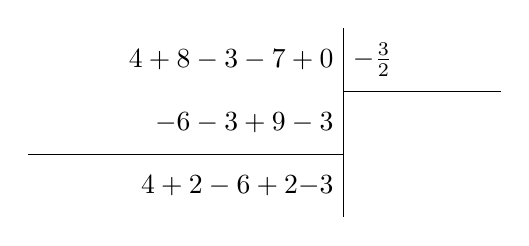
\begin{tikzpicture}[yscale=.8]
\node at (0,0)[left]{$4+8-3-7+0$};
\node at (0,-1)[left]{$-6-3+9-3$};
\node at (0,-2)[left]{$4+2-6+2\boxed{-3}$};
\draw (0,.5)--(0,-2.5);
\draw (0,-.5)--(2,-.5);
\draw (-4,-1.5)--(0,-1.5);
\node at (0,0)[right]{$-\frac{3}{2}$};
\end{tikzpicture}
\end{center}
所以$f(x)$除以$\left(x+\frac{3}{2}\right)$得商式$4x^3+2x^2-6x+2$,余式$-3$。即所求的商式为$q(x)=4x^3+2x^2-6x+2$,余式为$r(x)=-3$。
\end{solution}

容易看出以上两个例子中所得的结果,都符合带余除法恒等式
\[f (x) =q (x) \cdot g (x) +r (x) \]

一般地,多项式带余除法,有以下重要定理:

\begin{blk}{定理}
    对于任意两个多项式$f(x)$, $g(x)\ne 0$, 总是存在唯一的两个多项式$q(x),r(x)$, 使得等式
$f(x) =q(x)\cdot g (x) + r(x) $
成立,并且满足${\rm deg}r(x)<{\rm deg}g(x)$或$r(x)=0$。
\end{blk}

\begin{analyze}
    这个定理的内容既指出了$q(x),r(x)$的存在性——可以找到,又指出了$q(x),r(x)$对于给定的$f(x),g(x)\ne 0$是唯一的——没有第二个。因而,证明理应从这两个方面进行。
\end{analyze}

\begin{proof}
    先证存在性,可按$f(x),g(x)$的次数分为三种情况考虑。
\begin{enumerate}
    \item 若$f(x)=0$, 则不论$g(x)$是什么样的非零多项式,都
可以取$q(x)=r(x)=0$, 显然满足
\[f(x)=q(x)\cdot g(x)+r(x),\quad \text{且}r(x)=0\]
\item 若$f(x)\ne 0$, 且${\rm deg}f(x)<{\rm deg}g(x)$,则可取$q(x)=0$, $r(x)=f(x)$。同样满足
\[f(x)=q(x)\cdot g(x)+r(x),\quad \text{且}{\rm deg}r(x)<{\rm deg}g(x)\]
\item 若$f(x)\ne 0$, 且${\rm deg}f(x)\ge {\rm deg}g(x)$,则可以按下面的方法求出$q(x), r(x)$:

首先用$g(x)$的最高次项去除$f(x)$的最高次项,可得到商$q_1(x)$与余$f_1(x)$,使等式
\begin{equation}
    f (x) =q_1 (x)\cdot y(x)+f_1(x)
\end{equation}
成立,其中$f_1(x)$至少比$f(x)$降低一次,即${\rm deg}f_1(x)<{\rm deg}f(x)$,或$f_1(x)=0$。这时可能有两种情况出现:
\begin{enumerate}
    \item 若${\rm deg}f_1(x)<{\rm deg}g(x)$,或$f_1(x)=0$,我们就取
    \[q(x)=q_1(x),\qquad r(x)=f_1(x)\]
显然定理条件被满足;
\item 若${\rm deg}f_1(x)\ge {\rm deg}g(x)$, 我们就对$f_1(x)$与$g(x)$两个多项式去做上述同样的运算。
\end{enumerate}

其次用$g(x)$的最高次项去除$f_1(x)$的最高次项,可得到商式$q_2(x)$与余式$f_2(x)$, 使等式
\begin{equation}
    f_1(x)=q_2(x)\cdot g(x)+f_2(x)
\end{equation}
成立,其中$f_2(x)$的次数又至少比$f_1(x)$的次数降低一次,即${\rm deg}f_2(x)<{\rm deg}f_1(x)$,或$f_2(x)=0$,这时,
\begin{enumerate}
    \item 若${\rm deg}f_2(x)<{\rm deg}g(x)$,或$f_2(x)=0$,由(3.3)、(3.4)式得
    \[f(x)=[q_1(x)+q_2(x)]\cdot g(x)+f_2(x)\]
    我们就取$q(x)=q_1(x)+q_2(x),\quad r(x)=f_2(x)$。
    定理显然被满足;
    \item 若${\rm deg}f_2(x)\ge {\rm deg}g(x)$,就对$f_2(x)$与$g(x)$做上述同
样运算,同样可以将$f_2(x)$的次数降低至少一次,得到商式$q_3(x)$与余式$f_3(x)$,……作上述同样的分析、处理。
\end{enumerate}

再次,由于${\rm deg}f(x)$是一个非负整数,经过有限次的逐次至少减一,总会有一次(设第$k$次)达到${\rm deg}f_k(x)<{\rm deg}g(x)$或$f_k(x)=0$。于是,我们可得等式
\begin{equation*}
    f_{k-1}(x)=q_k(x)\cdot g(x)+f_k(x) \tag{$k$}
\end{equation*}

综上所述,由等式(3.3)、(3.4)、……($k$),就可以得到
\[\begin{split}
   f(x)&=q_1(x)\cdot g(x)+f_1(x)\\
   &=[g_1(x)+q_2(x)]\cdot g(x)+f_2(x)\\ 
&=\cdots\cdots\\
&=[q_1(x)+q_2(x)+\cdots+q_k(x)]\cdot g(x)+f_k(x)
\end{split}\]
其中,${\rm deg}f_k(x)<{\rm deg}g(x)$或$f_k(x)=0$。

这时,我们就取
\[\begin{split}
    q(x)&=q_1(x)+q_2(x)+\cdots +q_k(x)\\
    r(x)&=f_k(x)
\end{split}\]
显然,这样定理的条件被满足。存在性证毕。
\end{enumerate}

下面再证$q(x)$与$r(x)q$的唯一性。假设除$q(x),r(x)$外,还存在另外一组$q'(x),r'(x)$也满足
\begin{enumerate}
    \item $f(x)=q'(x)\cdot g(x)+r'(x)$,且${\rm deg}r'(x)<{\rm deg}g(x)$或$r'(x)=0$。结合已有的$q(x)$, $r(x)$满足。
    \item $f(x)=q(x)\cdot g(x)+r(x)$,且${\rm deg}r(x)<{\rm deg}g(x)$或$r(x)=0$就可以得出
\[q(x)\cdot g(x)+r(x)=q'(x)\cdot g(x)+r'(x)\]
所以
\[[q(x)-q'(x)]\cdot g(x)=r'(x)-r(x)\]
\end{enumerate}

在此等式中,如果$q(x)-q'(x)\ne 0$,则有
\[{\rm deg}\{[q(x)-q'(x)]\cdot g(x)\}\ge {\rm deg}g(x)\]
但是,由上面的情形又有
${\rm deg}[r'(x)-r(x)]<{\rm deg}g(x)$或$[r'(x)-r(x)]$不定义次数,这是不可能的。所以
\[q'(x)-q(x)=0\quad \Rightarrow\quad q'(x)=q(x)\]

又由于$g(x)\ne 0$,因而$r'(x)-r(x)=0$,即$r'(x)=r(x)$。因此,$q'(x)=q(x)$, $r'(x)=r(x)$。唯一性证毕。
\end{proof}

带余除法是一元多项式的特有运算,但对于二元齐次多项式,我们也可以把其中的一元看作常数来进行带余除法。但是,当余式不为零时,由于选作常数的元的不同,商式与余式也会不同的。

\begin{example}
 已知$f(x,y)=2x^3+7x^2y+13xy^2+5y^3$, $g(x,y)=2x+y$, 试求:
 \begin{enumerate}
     \item 把$y$看作常数时
     \item 把$x$看作常数时
 \end{enumerate}
$f(x,y)$除以$g(x,y)$所得的商式$q(x,y)$与余式$r(x,y)$。
\end{example}

\begin{solution}
\begin{center}
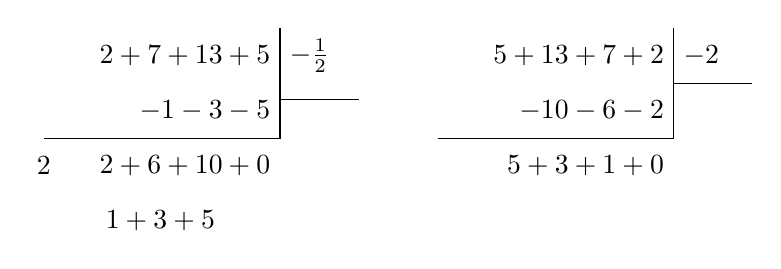
\begin{tikzpicture}[yscale=.7]
\begin{scope}
    \node at (0,0)[left]{$2+7+13+5$};
    \node at (0,-1)[left]{$-1-3-5$};
    \node at (0,-2)[left]{$\boxed{2+6+10}+0$};
    \node at (0,-3)[left]{$1+3+5\qquad $};
    \node at (0,0)[right]{$-\frac{1}{2}$};
    \node at (-3,-2){2};
    \draw (-3,-1.5)--(0,-1.5)--(0,.5);
    \draw (0,-.8)--(1,-.8);
\end{scope}
\begin{scope}[xshift=5cm]
    \node at (0,0)[left]{$5+13+7+2$};
    \node at (0,-1)[left]{$-10-6-2$};
    \node at (0,-2)[left]{$5+3+1+0$};
    \node at (0,0)[right]{$-2$};
    \draw (0,-.5)--(1,-.5);
    \draw (-3,-1.5)--(0,-1.5)--(0,.5);
\end{scope}
\end{tikzpicture}
\end{center}
\begin{enumerate}
    \item $q(x,y)=x^2+3xy+5y^2,\qquad r(x,y)=0$
    \item  $q(x,y)=5y^2+3xy+x^2,\qquad r(x,y)=0$
\end{enumerate}
\end{solution}

\begin{example}
已知$f(x,y)=2x^3+7x^2y+13xy^2+y^3$, $g(x,y)=2x+y$。要求同例3.7。
\end{example}

\begin{solution}
\begin{center}
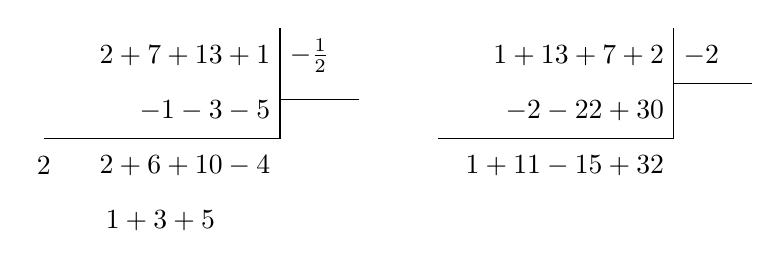
\begin{tikzpicture}[yscale=.7]
\begin{scope}
    \node at (0,0)[left]{$2+7+13+1$};
    \node at (0,-1)[left]{$-1-3-5$};
    \node at (0,-2)[left]{$\boxed{2+6+10}-4$};
    \node at (0,-3)[left]{$1+3+5\qquad $};
    \node at (0,0)[right]{$-\frac{1}{2}$};
    \node at (-3,-2){2};
    \draw (-3,-1.5)--(0,-1.5)--(0,.5);
    \draw (0,-.8)--(1,-.8);
\end{scope}
\begin{scope}[xshift=5cm]
    \node at (0,0)[left]{$1+13+7+2$};
    \node at (0,-1)[left]{$-2-22+30$};
    \node at (0,-2)[left]{$1+11-15+32$};
    \node at (0,0)[right]{$-2$};
    \draw (-3,-1.5)--(0,-1.5)--(0,.5);
    \draw (0,-.5)--(1,-.5);
\end{scope}
\end{tikzpicture}
\end{center}
\begin{enumerate}
    \item $q(x,y)=x^2+3xy+5y^2,\qquad r(x,y)=-4y^3$
    \item  $q(x,y)=y^2+11xy-15x^2,\qquad r(x,y)=32x^3$
\end{enumerate}
\end{solution}

\begin{ex}
\begin{enumerate}
    \item 若$n$次多项式$f(x)$除以$m$次多项式$g(x)$, 试确定所得商式和余式的次数。
    \item 求$f(x)$除以$g(x)$的商式$q(x)$及余式$r(x)$
\begin{enumerate}
    \item $f(x)=x^3+3x^2-x+7,\quad g(x)=x+2$
    \item $f(x)=x^3+3x^2-x+7,\quad g(x)=2x+1$
    \item $f(x)=4x^4+4x^3+5x^2+2x+1,\quad 
g (x) =2x^2+x+1$
    \item $f (x) =x^5+30a^5,\quad g (x) =x+2a$
    \item $f(x)=x^3+3ax^2+(2a^2 -a)x+(a-1),\quad g (x) =x+a-1$
    \item $f(x)=42x^9-13x^7-104x^5+84x^3+9x,\quad 
g (x) =6x^4+11x^2+1$
\end{enumerate}
\item 
若已知除式$g(x)=2x^2-x+3$, 商式$q(x)=x^2-5$, 余式$r(x)=3x+1$, 试求被除式$f(x)$。

\item 试任选一元作常数,求下列$f(x,y)$除以$g(x,y)$所得的商式与余式:
\begin{enumerate}
    \item $f (x,y) =2x^4-x^3y-2x^2y^2-2xy^3-y^4,\quad 
g (x,y) =2x^2+xy+y^2$
    \item $f(x,y)=2x-x^3y-2xy^3-y^4,\quad 
g (x,y) =2x^2+xy+y^2$
\end{enumerate}

\item 求$a^3-b^3+c^3+3abc$除以$a-b+c$所得的商式与余式。
\end{enumerate}
\end{ex}







